
\documentclass[conference]{IEEEtran}
\usepackage{color}

% *** MISC UTILITY PACKAGES ***
%
%\usepackage{ifpdf}
% Heiko Oberdiek's ifpdf.sty is very useful if you need conditional
% compilation based on whether the output is pdf or dvi.
% usage:
% \ifpdf
%   % pdf code
% \else
%   % dvi code
% \fi
% The latest version of ifpdf.sty can be obtained from:
% http://www.ctan.org/tex-archive/macros/latex/contrib/oberdiek/
% Also, note that IEEEtran.cls V1.7 and later provides a builtin
% \ifCLASSINFOpdf conditional that works the same way.
% When switching from latex to pdflatex and vice-versa, the compiler may
% have to be run twice to clear warning/error messages.

\usepackage{cite}
% cite.sty was written by Donald Arseneau
% V1.6 and later of IEEEtran pre-defines the format of the cite.sty package
% \cite{} output to follow that of IEEE. Loading the cite package will
% result in citation numbers being automatically sorted and properly
% "compressed/ranged". e.g., [1], [9], [2], [7], [5], [6] without using
% cite.sty will become [1], [2], [5]--[7], [9] using cite.sty. cite.sty's
% \cite will automatically add leading space, if needed. Use cite.sty's
% noadjust option (cite.sty V3.8 and later) if you want to turn this off.
% cite.sty is already installed on most LaTeX systems. Be sure and use
% version 4.0 (2003-05-27) and later if using hyperref.sty. cite.sty does
% not currently provide for hyperlinked citations.
% The latest version can be obtained at:
% http://www.ctan.org/tex-archive/macros/latex/contrib/cite/
% The documentation is contained in the cite.sty file itself.

\usepackage{hyperref}


% *** GRAPHICS RELATED PACKAGES ***
%
\ifCLASSINFOpdf
  \usepackage[pdftex]{graphicx}
  % declare the path(s) where your graphic files are
  % \graphicspath{{../pdf/}{../jpeg/}}
  % and their extensions so you won't have to specify these with
  % every instance of \includegraphics
  \DeclareGraphicsExtensions{.pdf,.jpeg,.png}
\else
  % or other class option (dvipsone, dvipdf, if not using dvips). graphicx
  % will default to the driver specified in the system graphics.cfg if no
  % driver is specified.
  % \usepackage[dvips]{graphicx}
  % declare the path(s) where your graphic files are
  % \graphicspath{{../eps/}}
  % and their extensions so you won't have to specify these with
  % every instance of \includegraphics
  % \DeclareGraphicsExtensions{.eps}
\fi
% graphicx was written by David Carlisle and Sebastian Rahtz. It is
% required if you want graphics, photos, etc. graphicx.sty is already
% installed on most LaTeX systems. The latest version and documentation can
% be obtained at:
% http://www.ctan.org/tex-archive/macros/latex/required/graphics/
% Another good source of documentation is "Using Imported Graphics in
% LaTeX2e" by Keith Reckdahl which can be found as epslatex.ps or
% epslatex.pdf at: http://www.ctan.org/tex-archive/info/
%
% latex, and pdflatex in dvi mode, support graphics in encapsulated
% postscript (.eps) format. pdflatex in pdf mode supports graphics
% in .pdf, .jpeg, .png and .mps (metapost) formats. Users should ensure
% that all non-photo figures use a vector format (.eps, .pdf, .mps) and
% not a bitmapped formats (.jpeg, .png). IEEE frowns on bitmapped formats
% which can result in "jaggedy"/blurry rendering of lines and letters as
% well as large increases in file sizes.
%
% You can find documentation about the pdfTeX application at:
% http://www.tug.org/applications/pdftex





% *** MATH PACKAGES ***
%
\usepackage[cmex10]{amsmath}
% A popular package from the American Mathematical Society that provides
% many useful and powerful commands for dealing with mathematics. If using
% it, be sure to load this package with the cmex10 option to ensure that
% only type 1 fonts will utilized at all point sizes. Without this option,
% it is possible that some math symbols, particularly those within
% footnotes, will be rendered in bitmap form which will result in a
% document that can not be IEEE Xplore compliant!
%
% Also, note that the amsmath package sets \interdisplaylinepenalty to 10000
% thus preventing page breaks from occurring within multiline equations. Use:
\interdisplaylinepenalty=2500
% after loading amsmath to restore such page breaks as IEEEtran.cls normally
% does. amsmath.sty is already installed on most LaTeX systems. The latest
% version and documentation can be obtained at:
% http://www.ctan.org/tex-archive/macros/latex/required/amslatex/math/










\usepackage[font=footnotesize,labelsep=period]{caption}
\renewcommand{\figurename}{Figure}
%\usepackage[font=footnotesize]{subfig}
% subfig.sty, also written by Steven Douglas Cochran, is the modern
% replacement for subfigure.sty. However, subfig.sty requires and
% automatically loads Axel Sommerfeldt's caption.sty which will override
% IEEEtran.cls handling of captions and this will result in nonIEEE style
% figure/table captions. To prevent this problem, be sure and preload
% caption.sty with its "caption=false" package option. This is will preserve
% IEEEtran.cls handing of captions. Version 1.3 (2005/06/28) and later
% (recommended due to many improvements over 1.2) of subfig.sty supports
% the caption=false option directly:
%\usepackage[caption=false,font=footnotesize]{subfig}
%
% The latest version and documentation can be obtained at:
% http://www.ctan.org/tex-archive/macros/latex/contrib/subfig/
% The latest version and documentation of caption.sty can be obtained at:
% http://www.ctan.org/tex-archive/macros/latex/contrib/caption/

\usepackage{fixltx2e}
\usepackage{stfloats}

%\usepackage{url}


% correct bad hyphenation here
\hyphenation{op-tical net-works semi-conduc-tor}

\usepackage{xcolor}
\usepackage{flushend}

\colorlet{pcolor}{blue}
\colorlet{fcolor}{red}
\newcommand{\e}[2][fcolor]{\textcolor{pcolor}{[}\textcolor{#1}{#2}\textcolor{pcolor}{]}}

\hypersetup{
    bookmarks=true,         % show bookmarks bar?
    unicode=true,           % non-Latin characters in Acrobat’s bookmarks
    pdftoolbar=true,        % show Acrobat’s toolbar?
    pdfmenubar=true,        % show Acrobat’s menu?
    pdffitwindow=false,     % window fit to page when opened
    pdfstartview={FitH},    % fits the width of the page to the window
    pdftitle={A Semantic Markup Technique Based on Ontology Polysystem},    % title
    pdfauthor={Evgeny Cherkashin, Kristina Paskal, Igor Bychkov},     % author
    pdfsubject={Scientific paper},   % subject of the document
    pdfcreator={LaTeX},   % creator of the document
    pdfproducer={LaTeX}, % producer of the document
    pdfkeywords={polysystem} {ontology} {semantic web} {knowledge
      acquisition} {data mining} {natural language processing}, % list of keywords
    pdfnewwindow=true,      % links in new window
    colorlinks=true,       % false: boxed links; true: colored links
    %linkcolor=[rgb]{0 0.4 0.1},          % color of internal links (black)
    linkcolor=black,          % color of internal links (black)
    %citecolor=blue,        % color of links to bibliography
    citecolor=black,        % color of links to bibliography
    filecolor=black,      % color of file links
    %urlcolor=[rgb]{0.3 0.0 0.3}           % color of external links
    urlcolor=black           % color of external links
}

\newenvironment{asdcode}{\hangindent=\parindent\hangafter=1\par\noindent\small\tt}{}


\begin{document}
\title{Information System Models for Support of Natural Language Question-Answering Subsystems Construction}
  \author{%
   \IEEEauthorblockN{%
    Alexey Hmelnov\IEEEauthorrefmark{1}\IEEEauthorrefmark{2},
    Evgeny Fereferov\IEEEauthorrefmark{1},
    Roman Fedorov\IEEEauthorrefmark{1}\IEEEauthorrefmark{2},
    Evgeny Cherkashin\IEEEauthorrefmark{1}\IEEEauthorrefmark{2}\IEEEauthorrefmark{3}, \\
    Polina Belykh\IEEEauthorrefmark{1},
    Alexander Zamashikov\IEEEauthorrefmark{3}
   }%
  \IEEEauthorblockA{\IEEEauthorrefmark{1}Institute of System Dynamics
    and Control Theory at SB RAS, Irkutsk, Lermontov str., 134,
    664033, Russia}%
  \IEEEauthorblockA{\IEEEauthorrefmark{2}Irkutsk State University,
    Irkutsk, Gagarina blvd., 664003, Russia}%
  \IEEEauthorblockA{\IEEEauthorrefmark{3}National Research Irkutsk
    State Technical University, Irkutsk, Lermontov str., 83, 664074,
    Russia}%
\texttt{\small alex@icc.ru, fereferov@icc.ru, fedorov@icc.ru, eugeneai@icc.ru}
}

% use for special paper notices
%\IEEEspecialpapernotice{(Invited Paper)}

% make the title area
\maketitle

\def\thepage{Page \arabic{page}}
%\setcounter{page}{252}

\begin{abstract}
Software development technologies evolved from concrete algorithm design and their programmatic implementation to modeling the whole information systems (IS).  The modeling approaches allows developers to describe the system in terms of domain, design and features of implementation platforms, and standard ways of the IS development like programming traditions in a concrete firm.  In the case if a new IS is being constructed, having an already designed and realized database, Data Driven Engineering (DDE) is used.  The model of new IS is constructed by importing database structure and adding a semantic layer description reflecting the database structure to the domain terms.

We describe a DDE approach based on declarative specifications of existing database schema and properties of the target application, as well as interpretation of the description into IS components.  The interpretation in various aspects allows developer to construct user interface of database modification, subsystem of SQL query construction in terms of domain, etc.
\e{The report describes an approach of such kind of natural question-answering subsystem implementation for IS.  Examples of domain description has been presented for practical problems of municipal management.}

%The obtained description could be used to extend the capabilities of SQL query constructor to allow user formulating the query in a natural language, e.g. in Russian.  In order to do so a new layer of the domain and IS properties description should be devised.  The layer is based on an ontological description of the domain referencing the terms of the database description.  The layer also is to be reflected to morphological structures of the natural language used to formulate the queries.
\end{abstract}


% For peer review papers, you can put extra information on the cover
% page as needed:
% \ifCLASSOPTIONpeerreview
% \begin{center} \bfseries EDICS Category: 3-BBND \end{center}
% \fi
%
% For peerreview papers, this IEEEtran command inserts a page break and
% creates the second title. It will be ignored for other modes.
\IEEEpeerreviewmaketitle



\section{Introduction}
% no \IEEEPARstart
Software development technologies evolved from concrete algorithm design and their programmatic implementation to modeling the whole information systems (IS).  The modeling approaches allows developers to describe the system in terms of domain, engineering and software design and features of implementation platforms, and standards of the IS development of a software firm such as programming traditions, used modeling and instrumental tools, etc.  \e{Some more text transit from trends to their real implementations, like Group of a Senior Proggemmer, Extreme and Agile programming. Examples like Django..}

The theoretical basis of the development process is model transformation theories and their software implementations, which are developed in the field of Model Driven Engineering (MDE).  The transformations construct ultimately either source code modules realizing modeled structures or an operator interpretation of models of an intermediate level like virtual machine byte code, SQL queries \e{realization}, and executable UML. \e{\ldots{}}.

In the case if a new IS is being constructed, having already designed and deployed database, Data Driven Engineering (DDE, a kind of MDE) is widely used.  The model of new IS is constructed by importing database structure, e.g. DDL-queries, and adding a semantic layer of the database structure description in IS domain terms.  In laboratory of Complex Information Systems of Institute of System Dynamics and Control Theory at Siberian Branch of Russian Academy of Sciences, a number of DDE approaches has been developed based on declarative specifications and their run time interpretations, as well as techniques automating the description process.  The interpretation in various aspects allows developer to construct user interface of database modification, subsystem of SQL-queries construction in terms of domain, etc.

The obtained description could be used to extend the capabilities of SQL-query constructor to allow user formulating the query in a natural language, e.g. in Russian, in terms of modeled domain.  In order to do so a new layer of the domain and IS properties description should be devised.  The layer expands the description of the database entities and their relationships with abstract notions of domain and relations, resulting in fibered representation of the domain of two fibers: abstract domain and database structure.  The notions and relations are mapped through the fibers via interpretation.  \e{The layer is based on an ontological description of the domain referencing the terms of the database description.  The layer also is to be reflected to morphological structures of the natural language used to formulate the queries.}

The report describes an approach of such kind of natural question-answering subsystem implementation for IS.  Examples of domain description has been presented for practical problems of municipal management. \e{Some word about the problem...}

\e{In this paper, we continue the development of the approach
\cite{fereferovDiss} within the theoretical aspect \cite{b2:15} of software unified model development, and briefly consider the approach of unification of software modeling and natural language processing.}

\section{A Description of a Database/ The Description Language}
\label{sec:description-database}

Data Driven Engineering (DDE) \cite{DDE} one of the powerful direction of Computer science allowing to construct software on the base of data models (data structure description).  Being a part of Model Driven Engineering, DDE inherits its main thesis that software development is a sequence of model transformations starting from abstract models describing information system (IS) in terms of domain \e{and software development process}.

DDE starts either from description of a general view of data structures used by business-logic or from already existing database.  The second case has important value in practice, when customer requires a new implementation of an exiting IS with new features and with conserving exiting data in its warehouse.  ....

The structural description allows developers via transformation to implement routine functionality of IS such as data input forms; user interface and business-logic interaction; import, export and integration operations; etc.  Adding a domain description allows ones to refine user interface with notions familiar to user, as well as construct various query-answering subsystems like SQL-query builders and OLAP operating in terms of domain.

In Institute of System Dynamics and Control Theory at SB RAS a number of DDE technologies has been developed within economic contracts activities supported by necessary theoretical investigations.  One of the last description format is based on mix of the \texttt{.ini}-file and SQL-query languages.  The first format is used to describe database structure and semantic of attributes and their relations, the second part is used to describe the rules of user interface generation, and interaction with geographical information systems and other applications.

\subsection{Developing IS with Specifications}
\label{sec:descr-synth-stag}

In a general case on the first stage of IS development, system engineer carries on structural analysts of the domain, resulting in description of concepts and their basic relations, business-processes and software requirements.  After that, the database design follows, which produces database schema ad its implementation as database server.  Common design tools (such as Sybase Power Designer, IBM Rational Rose) are used on this stage.

On the third stage model of IS is constructed by loading the implemented database schema and extending it with the description of the following special database object classes: \texttt{table}, \texttt{view}, \texttt{rule}, and so called \texttt{superstructure}.  The \texttt{table} objects describe IS database structure and relations, attribute data types and names.  These object are automatically constructed by loading and analyzing IS database schema, if it is literally devised (it must be at least in third normal form).  The lack of schemata data is compensated manually with \e{the description language} and the following interpretation.

The \texttt{view} objects are more complicated than \texttt{tables} and used to generate user interface.  Here we define properties of the relation, for example, for each foreign key a loookup widget can be used to select a  record from a foreign table (a reference book).  For complex reference book and transitive references, the identification attribute set bust be specified to increase generated user interface usability.  There are other special cases of foreign key interpretations, like ``master-details'', and all of them can be specified with \e{the description language}.

The \texttt{superstructure} objects support interaction of developed IS with foreign modules and libraries processing information with methods beyond the standard of rational databases and SQL, e.g., computer simulation and complex data visualizations.

%\hangindent=\parindent%\hangafter=1
The \texttt{rules} objects are responsible for specific to business-processes functions implementation in generated IS.  By means of the rules, one can describe input field logic (enabling and disabling them), implement uniqueness check routines and \e{PD} interaction, i.e., rules provide declarative means of describing and implementing relationships between in business-logic layer of IS.  The rules also affect the generated queries to IS database during editing and creating special widgets in user interface, which connect input data with spatial tables and render cartographic.

\e{For all the object classes a formal set model is devised.  We will not describe it in this paper, ...}

On the forth stage the IS is generated as a result of the description interpretation.  It integrates according to the rules the foreign software subsystems. \e[blue]{Should we describe the rules of interface generation in details ?}

\subsection{The Description Language}

... The language has LL(1) grammar class.  Its syntactic structures describe elements of IS and a general options like database connection properties.  The specifications written in the language are \emph{precise}, \emph{understandable} and \emph{complete} according to [1,2].  The language clauses have the following general structure:

\begin{asdcode}%
<Start keyword> <List of mandatory statements> [~list of optional statements~]
\end{asdcode}

The \texttt{start keyword} can be one of the following: \texttt{ADO}, \texttt{BDE}, \texttt{CFG}, \texttt{Table}, \texttt{View}, \texttt{Plugins}, \texttt{Uses}, \texttt{Include}, \texttt{Menu}.  First two are used to describe properties of database connection.  Keyword \texttt{CFG} used to describe general application settings of IS.  Keywords \texttt{Table}, \texttt{View} describe the database schema and view widgets.  Keyword \texttt{Plugins} describes interaction with outer systems, \texttt{Uses} and \texttt{Include} allow developer to break an IS description into source modules.  Keyword \texttt{Menu} controls the main menu of IS application.

Let's consider a part of an example description.

\begin{asdcode}%
\textbf{TABLE} ADR \textbf{FOR} SP\_ADDR \textbf{AS} 'Address' \textbf{READONLY}
\end{asdcode}







\section{Interpretations of the Description}
\label{sec:interpr-descr}

\e[gray]{Describe a general approach to interpretation process.}

\subsection{User-Interace Form Generation}
\label{sec:user-interace-form}
One of the important IS quality characteristic is its input forms.  The layouting the widgets in forms is the question of the usability.  From one hand side the widgets must efficiently consume the form area of the form, and from another hand side the user interface must be convenient and fit to the application functionality requirements.

The variation of form size results in relayouting the widgets if the form is aware of the variation.  Various instrumental systems resolves the problem differently.  E.g., in Embarcadero Delphi developer must specify \texttt{align}, \texttt{anchors} and \texttt{autosize} properties to adjust the widgets behavior upon form size change.  The operation must be performed for each widget, and in conditions of entering of a database record of many attributes the adjustment process becomes somewhat problematic.  In addition, layout mechanics of Delphi cannot distribute the size variations between inside widgets proportionally.

The problem is solved in, e.g., open-source widget libraries, like Qt and GTK+.  The widgets are placed in so called containers (which are also a virtual widgets), which manage the order, spacing, padding, fill and expansion properties.  GTK+ widgets could also issue \texttt{size request} message to notify parent widget about required minimal size.  Nevertheless the general engines implemented in the instrumental systems are no aware of the attribute data properties of the IS database.

To account the properties, an rule based engine has been developed on the base of the database description.  ....


In comparison to Microsoft Access the developed layout engine, which also generated user interface on the base of database structure description, the engine ....

\subsection{On-Line Analitical Processing}
\label{sec:olap}

The IS description used to implement import routines for On-Line Analitical Processing unit (OLAPu).  The unit allows user to store, select and analyze numberic indicators.  The indicators are considered as funtions of a set of attributes.  OLAPu can 
selected the indicators in various projection combinations.  

OLAPu's design is classic client-server architecture, where server is a rational data storage, and client provide a flexible access to the indicator data by means of intuitive user interface.  The interface is configured specially to support the munidimentional OLAP.  The user by means of widgets of the interface selects and ajusts projection and indicator aggregation configuration, the results of the configuration are presented ast interactive tables and can be stored in Microdoft Excel spreadsheet pages.



\section{GIS Integration}
\label{sec:gis-integration}



\section{Query Builder}
\label{sec:query-builder}


Query constructor of Microsoft Access allows user to design a complex SQL-queries for aggregating and modifying data.  The query builder supports definition of complex conditions for the \texttt{WHERE} and \texttt{HAVING} sections of the query.  The query builder also does not account the domain, and, thus, it is intended for programmers and experienced users accounted with database technologies.  Another problem is the availability of the SQL-query designers for web projects.


\section{Natural Language Processing [within the problem]}
\label{sec:natur-lang-proc}

\section{Query Synthesis [NG]}
\label{sec:query-synthesis-ng}


\begin{figure}
\centering\footnotesize\sf
\def\svgwidth{0.9\linewidth}
\input{layer_en.pdf_tex}
\caption{A Usage Example of an Ontology Polysystem}
\label{OPSA}
\end{figure}

\begin{figure}[!t]
\centering
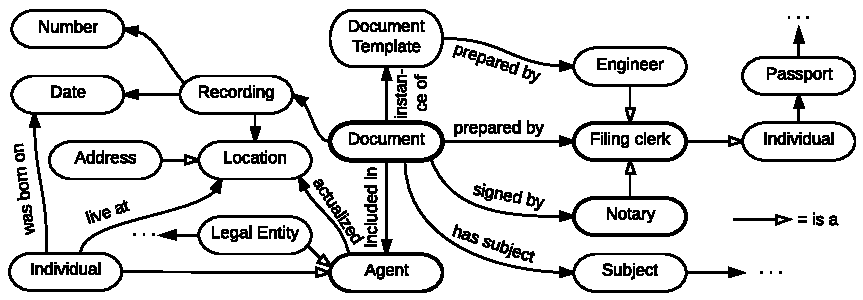
\includegraphics[width=\linewidth]{DocumentOntology-en.pdf}
% where an .eps filename suffix will be assumed under latex,
% and a .pdf suffix will be assumed for pdflatex; or what has been declared
% via \DeclareGraphicsExtensions.
\caption{Upper Layer of Notary Office Ontology}
\label{notaryontology}
\end{figure}


% A further development of the project is aimed at implementation of cognitive data mining (data analysis) in similar documents to reveal patterns between attributes that appear in the documents. The results of the analysis may be a basis of automation of document data storage technique decision. For example, if a set of attributes shows a strong correlation to an attribute than it can be interpreted as a relation of a relational database. The set forms a determinant (the key set of a table) and the set of strongly correlated attributes forms rest of the table as described in the Method of Functional Dependency. The method used by database engineers in the process of a database design, the dependencies revealed from the analysis of the attributes’ semantics. That is, the method could be used conversely, the dependencies can be revealed on the base of data mining.
% The abstract layer of information modeling of the knowledge acquisition is a category of system complexes (configurations) \cite{b2:15}, which is perfectly embody common metamodel of the ontologies as well as supply additional structural and functional properties. Developing the theory further one can connect the ontology devised during the document preparation process to the stage of UML-modelling of information system, which automates the processes of the domain.

%\subsubsection{Subsubsection Heading Here}
%Subsubsection text here.




% An example of a floating figure using the graphicx package.
% Note that \label must occur AFTER (or within) \caption.
% For figures, \caption should occur after the \includegraphics.
% Note that IEEEtran v1.7 and later has special internal code that
% is designed to preserve the operation of \label within \caption
% even when the captionsoff option is in effect. However, because
% of issues like this, it may be the safest practice to put all your
% \label just after \caption rather than within \caption{}.
%
% Reminder: the "draftcls" or "draftclsnofoot", not "draft", class
% option should be used if it is desired that the figures are to be
% displayed while in draft mode.
%

% Note that IEEE typically puts floats only at the top, even when this
% results in a large percentage of a column being occupied by floats.


% An example of a double column floating figure using two subfigures.
% (The subfig.sty package must be loaded for this to work.)
% The subfigure \label commands are set within each subfloat command, the
% \label for the overall figure must come after \caption.
% \hfil must be used as a separator to get equal spacing.
% The subfigure.sty package works much the same way, except \subfigure is
% used instead of \subfloat.
%
%\begin{figure*}[!t]
%\centerline{\subfloat[Case I]\includegraphics[width=2.5in]{subfigcase1}%
%\label{fig_first_case}}
%\hfil
%\subfloat[Case II]{\includegraphics[width=2.5in]{subfigcase2}%
%\label{fig_second_case}}}
%\caption{Simulation results}
%\label{fig_sim}
%\end{figure*}
%
% Note that often IEEE papers with subfigures do not employ subfigure
% captions (using the optional argument to \subfloat), but instead will
% reference/describe all of them (a), (b), etc., within the main caption.


% An example of a floating table. Note that, for IEEE style tables, the
% \caption command should come BEFORE the table. Table text will default to
% \footnotesize as IEEE normally uses this smaller font for tables.
% The \label must come after \caption as always.
%
%\begin{table}[!t]
%% increase table row spacing, adjust to taste
%\renewcommand{\arraystretch}{1.3}
% if using array.sty, it might be a good idea to tweak the value of
% \extrarowheight as needed to properly center the text within the cells
%\caption{An Example of a Table}
%\label{table_example}
%\centering
%% Some packages, such as MDW tools, offer better commands for making tables
%% than the plain LaTeX2e tabular which is used here.
%\begin{tabular}{|c||c|}
%\hline
%One & Two\\
%\hline
%Three & Four\\
%\hline
%\end{tabular}
%\end{table}


% Note that IEEE does not put floats in the very first column - or typically
% anywhere on the first page for that matter. Also, in-text middle ("here")
% positioning is not used. Most IEEE journals/conferences use top floats
% exclusively. Note that, LaTeX2e, unlike IEEE journals/conferences, places
% footnotes above bottom floats. This can be corrected via the \fnbelowfloat
% command of the stfloats package.


\section{Conclusion}

The nowadays techniques of application software development are aimed at close cooperation of developer and customer.  To shift some responsibility to the customer's users and to extend the maintainability and usability of software, it is necessary to develop a techniques, which produce some processing according to a domain description.  ...


% conference papers do not normally have an appendix

% use section* for acknowledgement
\section*{Acknowledgment}
The research is carried on under support of Integration multidisciplinary project of Siberian Branch of Russian Academy of Sciences N 17 “Development of services and infrastructure of scientific spatial data for supporting complex multidisciplinary scientific research of Baikal nature territory”.

%The authors would like to thank...

% trigger a \newpage just before the given reference
% number - used to balance the columns on the last page
% adjust value as needed - may need to be readjusted if
% the document is modified later
%\IEEEtriggeratref{8}
% The "triggered" command can be changed if desired:
%\IEEEtriggercmd{\enlargethispage{-5in}}

% references section

% can use a bibliography generated by BibTeX as a .bbl file
% BibTeX documentation can be easily obtained at:
% http://www.ctan.org/tex-archive/biblio/bibtex/contrib/doc/
% The IEEEtran BibTeX style support page is at:
% http://www.michaelshell.org/tex/ieeetran/bibtex/
%\bibliographystyle{IEEEtran}
% argument is your BibTeX string definitions and bibliography database(s)
%\bibliography{IEEEabrv,../bib/paper}
%
% <OR> manually copy in the resultant .bbl file
% set second argument of \begin to the number of references
% (used to reserve space for the reference number labels box)
\urlstyle{tt}
\vspace{1.4em} % For no reason the reference was sticked to the
               % previous paragraph
\begin{thebibliography}{11}
\bibitem{TBL2001} T.~Berners-Lee, J.~Hendler, O.~Lissila. ``The
  Semantic Web A new form of Web content that is meaningful to
  computers will unleash a revolution of new possibilities,''
  Scientific American, May 17, 2001,
  pp.~1-18. URL:~\url{http://sciam.com/article.cfm?articleID=00048144-10D2-1C70-84A9809EC588EF21}
\bibitem{father} A.~K.~Cherkashin. ``Polysystem Analysis and
  Synthesis. Application in Geography,'' Novosibirsk, Russia ``Nauka'' Publ. co.
  1997. -- 502~p. (In Russian)
\bibitem{SN} Social network -- Wikipedia, the free encyclopedia.
  URL:~\url{http://en.wikipedia.org/wiki/Social_network} (access date: 09.01.2015).
\bibitem{prevwork} E.~Cherkashin, P.~Belykh, D.~Annenkov, K.~Paskal, ``A
  Document Content Logical Layer Induction on the Base of Ontologies
  and Processing Changes,'' Procs. of International Conference on
  Applied Internet and Information Technologies, October 25, 2013,
  University of Novi Sad, Technical Faculty ``Mihajlo Pupin'',
  Zrenjanin, Republic of Serbia,
  pp.~252--257. URL:~\url{http://www.tfzr.uns.ac.rs/aiit/archives/AIIT2013/Proceedings.pdf}.
\bibitem{b2:15} E.~Cherkashin, V.~Paramonov, et al, ``Model Driven
  Architecture is a Complex System,'' E-Society Journal Research and
  Applications. Volume 2, Number 2, 2011, pp.~15--23.
  URL:~\url{http://www.tfzr.uns.ac.rs/esociety/issues/eSocietyVol2No2.pdf} (access date: 09.01.2015).
\bibitem{b2:5} Model--view--controller --- Wikipedia, the free
  encyclopedia.
  URL:~\url{http://en.wikipedia.org/wiki/Model-view-controller} (access date: 09.01.2015.)
\bibitem{diff} D.~MacKenzie, P.~Eggert, R.~Stallman. ``Comparing and Merging Files,''
  URL:~\url{http://www.gnu.org/software/diffutils/manual/diffutils.pdf} (access date: 09.01.2015).
\bibitem{dectrees} Information gain in decision trees ---  Wikipedia, the free
  encyclopedia. URL:~\url{http://en.wikipedia.org/wiki/Information_gain_in_decision_trees}
\bibitem{zopetal} ``Zope Page Templates Reference,'' The Zope2 Book. URL:~\url{http://docs.zope.org/zope2/zope2book/index.html} (access date: 09.01.2015).
\bibitem{cham} Chameleon -- Chameleon 2.10 documentation.
  URL:~\url{http://chameleon.readthedocs.org/en/latest/}  (access date: 09.01.2015).
\bibitem{kiyoto} Kyoto Cabinet. URL:~\url{http://fallabs.com/kyotocabinet/} (access date: 09.01.2015).
\bibitem{mediawiki}
 Semantic MediaWiki. URL: \url{http://semantic-mediawiki.org/} (access date: 20.08.2013).
\bibitem{heino}
 N.Heino, S.Tramp, N.Heino, S.Auer. Managing Web Content using Linked Data Principles – Combining semantic structure with dynamic content syndication. Computer Software and Applications Conference (COMPSAC), 2011 IEEE 35th Annual. pp. 245 - 250. URL:\url{http://svn.aksw.org/papers/2011/COMPSAC_lod2.eu/public.pdf} (access date: 30.05.2013).

\end{thebibliography}
\vspace{-2em}\mbox{} %Make the flushend work correctly with the last \bibitem
% that's all folks
\end{document}

%%% Local Variables:
%%% mode: latex
%%% TeX-master: t
%%% End:
